\documentclass[11pt]{report} %tamaño de letra, tipo de papel, tipo de documento
\usepackage{geometry}
\geometry{
	 a4paper,
	 total={210mm,297mm},
	 left=40mm,
	 right=20mm,
	 top=40mm,
	 bottom=30mm,
 }
\usepackage[spanish]{babel} %Reconocimento del español
\usepackage[utf8]{inputenc} %Reconocimento de la tilde
\usepackage{amsmath} %Insertar fórmulas matemáticas
\usepackage{amsfonts}
\usepackage{graphicx} %Paquete para incluir gráficos en el documento
\usepackage{caption} %Paquete para referenciar imágenes
\usepackage{refstyle} %Paquete para referencias cruzadas
\usepackage{comment} %Para los comentarios
\usepackage{natbib} %Para las bibliografias
%\usepackage{hyperref}
\usepackage[T1]{fontenc}
\usepackage{textcomp} %Para los simbolos de (R) y TM

\usepackage{longtable} %Paquete para lista de simbolos

%Paquete para columnas y texto vertical 
\newcommand*\rot{\rotatebox{90}}
\newcommand*\OK{\ding{51}}

%\usepackage{array}
\usepackage{makecell}

\renewcommand\theadalign{cb}
\renewcommand\theadfont{\bfseries}
\renewcommand\theadgape{\Gape[4pt]}
\renewcommand\cellgape{\Gape[4pt]}

\usepackage{multirow}
\usepackage{float}

\usepackage{listings} % Paquete para escribir programas

\setlength\parindent{0pt} %Para quitar la sangría al inicio de los parrafos

\title{Informe de laboratorio 4 de Robótica industrial} % Title

\author{Juan Diego \textsc{Cárdenas}} % Author name

\date{\today} % Date for the report

\begin{document}

	\maketitle

	\section{Introducción}
	En el presente informe se mostrará la metodología y los resultados del laboratorio 4 de la asignatura de robótica industria, la cual se enfocó en el estático de un robot planar de 3 grados de libertad, así como también, la simulación de un control resolved-rate para manipular las velocidades de los actuadores rotacionales, por último se describirá los efectos que posee el movimiento del robot sobre la matriz Jacobiana y su determinante.

	\section{Condiciones iniciales del Robot}
	En esta sección se describirán las condiciones iniciales con las que el robot trabajado fue implementado. En la Figura \ref{Figura: Robot} se pueden observar los parámetros del robot tales como las distancias de los eslabones y las variables de control ${\theta}_{1}$, ${\theta}_{2}$ y ${\theta}_{3}$, las cuales hacen referencia al angulo de giro de los ejes del robot.

	\begin{figure}[H]
		\centering
		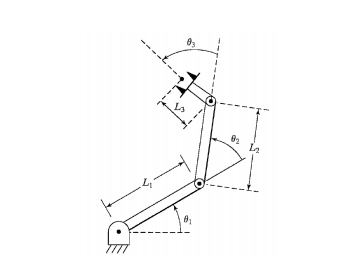
\includegraphics[width=10cm]{Imagenes/Robotinit.png}
		\caption{Robot planar de 3 grados de libertad, imagen tomada de \cite{Jaramillo2015}}
		\label{Figura: Robot}
	\end{figure}

	En la tabla \ref{Tabla: Longitudes}, se muestran los valores numéricos de las longitudes del robot.

	\begin{table}[]
		\centering
		\begin{tabular}{|c|c|}
			\hline
			\textbf{Variable} & \textbf{Valor} \\ \hline
			L1                & 4 m                     \\ \hline
			L2                & 3 m                     \\ \hline
			L3                & 2 m                     \\ \hline
		\end{tabular}
		\caption{Longitudes de los eslabones}
		\label{Tabla: Longitudes}
	\end{table}

	Seguido a esto, en la tabla \ref{Tabla: Angulos}, se muestran los valores iniciales de los ángulos de las articulaciones del robot.

	\begin{table}[]
		\centering
		\begin{tabular}{|c|c|}
			\hline
			\textbf{Variable} & \textbf{Valor} \\ \hline
			${\theta}_{1}$    & $10º$                  \\ \hline
			${\theta}_{2}$    & $20º$                  \\ \hline
			${\theta}_{3}$    & $30º$                  \\ \hline
		\end{tabular}
		\caption{Ángulos iniciales de las articulaciones}
		\label{Tabla: Angulos}
	\end{table}

	Así mismo, en la tabla \ref{Tabla: Velocidades}, se muestran los valores iniciales de las velocidades del extremo del robot.

	\begin{table}[]
		\centering
		\begin{tabular}{|c|c|}
			\hline
			\textbf{Variable}  & \textbf{Valor}  \\ \hline
			$\dot{X}$          & $0.2  m/s  $    \\ \hline
			$\dot{Y}$          & $-0.3 m/s  $    \\ \hline
			${\omega}_{z}$     & $-0.2 rad/s$    \\ \hline
		\end{tabular}
		\caption{Velocidades iniciales de las articulaciones}
		\label{Tabla: Velocidades}
	\end{table}

	A continuación, se plantea que la matriz Jacobiana del robot planar viene dada por la matriz $J$. Por último, en la tabla \ref{Tabla: Fuerzas}, se muestran las fuerzas y los torques del extremo del robot.
%
%	\begin{equation}
%		J = 
%		\begin{bmatrix}
%			-L1*sin({q}_{1})-L2*sin({q}_{1} + {q}_{2})-L3*sin({q}_{1} + {q}_{2} + {q}_{3}) & -L2*sin({q}_{1} + {q}_{2})-L3*sin({q}_{1} + {q}_{2} + {q}_{3}) & -L3*sin({q}_{1} + {q}_{2} + {q}_{3})\\
%        	 L1*cos({q}_{1})+L2*cos({q}_{1} + {q}_{2})+L3*cos({q}_{1} + {q}_{2} + {q}_{3}) &  L2*cos({q}_{1} + {q}_{2})+L3*cos({q}_{1} + {q}_{2} + {q}_{3}) &  L3*cos({q}_{1} + {q}_{2} + {q}_{3})\\
%          	 1 &                                                1 &                                     1                         
%		\end{bmatrix}
%		\label{Ecuacion: Jacobiano}
%	\end{equation}	



	\begin{table}[H]
		\centering
		\begin{tabular}{|c|c|}
			\hline
			\textbf{Variable}  & \textbf{Valor}  \\ \hline
			$\dot{X}$          & $0.2  m/s  $    \\ \hline
			$\dot{Y}$          & $-0.3 m/s  $    \\ \hline
			${\omega}_{z}$     & $-0.2 rad/s$    \\ \hline
		\end{tabular}
		\caption{Fuerzas y los torques del extremo del robot}
		\label{Tabla: Fuerzas}
	\end{table}

	\section{Trayectoria del robot}

	La trayectoria del robot fue calculada acorde al control resolved-rate, planteado en la figura \ref{Figura: Control}. 

	\begin{figure}[H]
		\centering
		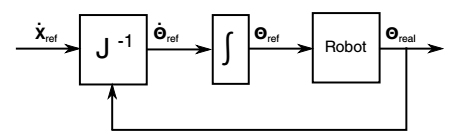
\includegraphics[width=10cm]{Imagenes/control.png}
		\caption{Diagrama de bloques para el control del robot}
		\label{Figura: Control}
	\end{figure}

	Siendo el elemento ${J}^{-1}$ el inverso de la matriz Jacobiana mostrada en la ecuación \ref{Ecuacion: Jacobiano}, y el elemento integrador hace referencia a la ecuación \ref{}

	\begin{equation}
		{\theta}_{i + 1} = {\theta}_{i} + {\dot{\theta}}_{i} \Delta
	\end{equation}

	La trayectoria resultante del procedimiento planteado se muestra en la figura \ref{Figura: Trayectoria}

	\begin{figure}[H]
		\centering
		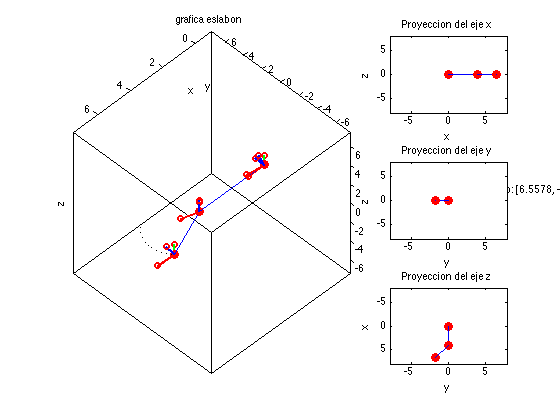
\includegraphics[width=10cm]{Imagenes/robot.png}
		\caption{Trayectoria generada por el robot manipulador}
		\label{Figura: Trayectoria}
	\end{figure}

	\section{Coordenadas articulares del robot}

	En la figura \ref{Figura: angulo}, se muestran las coordenadas articulares del robot, en donde se puede observar el comportamiento independiente de cada articulación del robot; estos ángulos fueron calculados usando el control planteado en la figura \ref{Figura: Control}.

	\begin{figure}[H]
		\centering
		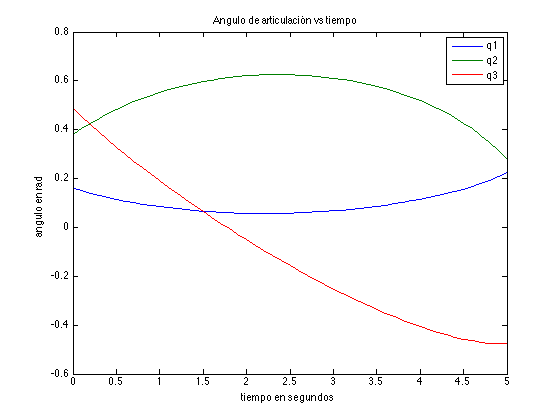
\includegraphics[width=10cm]{Imagenes/angulo.png}
		\caption{Coordenadas articulares del robot en radianes}
		\label{Figura: angulo}
	\end{figure}

	\section{Velocidades articulares del robot}

	Las velocidades de las articulaciones del robot fueron calculadas de acuerdo a la ecuación \ref{Ecuacion: Velocidad}, siendo $Q$ el vector de las velocidades de las articulaciones, $J$ la matriz Jacobiana y $\dot{X}$ el vector de velocidades del actuador final.

	\begin{equation}
		Q = {J}^{-1}\dot{X}
		\label{Ecuacion: Velocidad}
	\end{equation}

	Los resultados de la simulación se muestran en la figura \ref{Figura: Velocidad}.

	\begin{figure}[H]
		\centering
		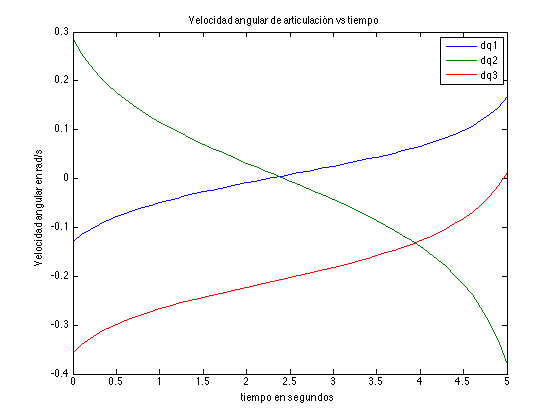
\includegraphics[width=10cm]{Imagenes/velocidades.png}
		\caption{Velocidades articulares del robot}
		\label{Figura: Velocidad}
	\end{figure}

	\section{Coordenadas cartesianas del extremo del robot}

	Después de calcular las coordenadas articulares de las articulaciones, se procede a calcular la posición del extremo del robot a partir de la transformada cinemática directa, la cual proviene de los parámetros de Denavit - Hartenberg (D - H), los resultados de la simulación se muestran en la figura \ref{Figura: extremo}.

	\begin{figure}[H]
		\centering
		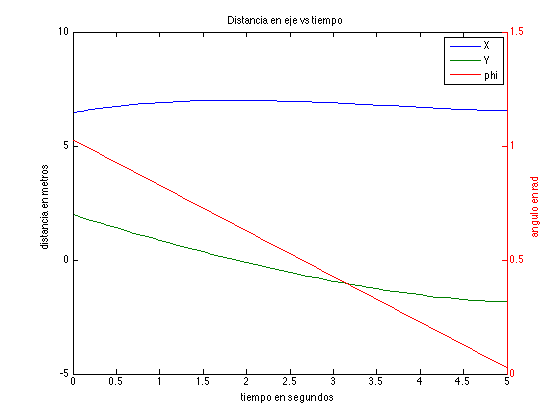
\includegraphics[width=10cm]{Imagenes/distancia.png}
		\caption{Coordenadas cartesianas del extremo del robot}
		\label{Figura: extremo}
	\end{figure}

	\section{Torques de las articulaciones del robot}

	Posteriormente, se procede a calcular los torques de las articulaciones del robot, haciendo uso de la ecuación \ref{Ecuacion: torque}, en donde $\tau$ hace referencia al vector de torques en las articulaciones, $J$ es la matriz Jacobiana y $W$ es el vector de fuerzas y torques del extremo del robot.

	\begin{equation}
		\tau = {J}^{T}W
		\label{Ecuacion: torque}
	\end{equation}

	Los resultados de la simulación se muestran en la figura \ref{Figura: torque}

	\begin{figure}[H]
		\centering
		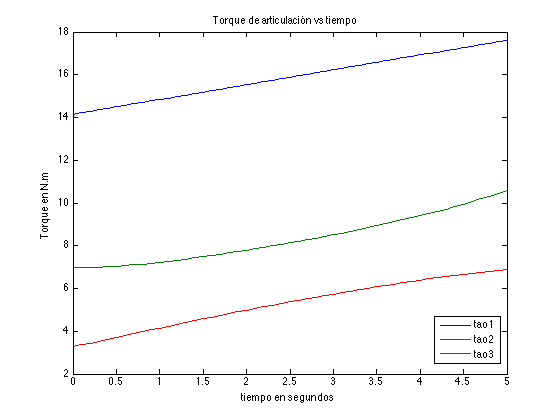
\includegraphics[width=10cm]{Imagenes/torque.png}
		\caption{Torques de las articulaciones del robot}
		\label{Figura: torque}
	\end{figure}

	\section{Matriz Jacobiana}

	En la figura \ref{Figura: Jacobiano}, se puede observar en un primer momento un incremento del determinante de la matriz Jacobiana, lo cual se debe al movimiento de extención que está realizando el robot, hay que precisar que con este movimiento, el robot se acerca a uno de sus puntos singulares, en el puede estar fuera de su espacio de trabajo.

	\begin{figure}[H]
		\centering
		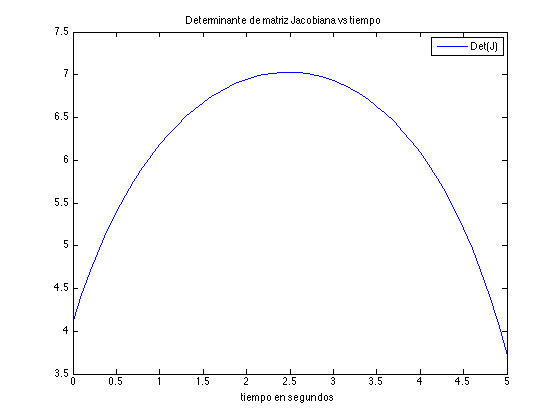
\includegraphics[width=10cm]{Imagenes/detJ.png}
		\caption{Evolución del determinante de la matriz Jacobiana en la trayectoria del robot}
		\label{Figura: Jacobiano}
	\end{figure}

	Por otra parte, las zonas de los mínimos locales de la gráfica pueden ser relacionados a un aumento de la aceleración, reflejado en el mismo periodo de tiempo en la figura \ref{Tabla: Velocidades}, y mientras que se acerca al máximo local, la aceleración tiende a disminuir.\\

	Por último, respecto a los torque mostrados en la figura \ref{Tabla: torque}, se puede apreciar que conforme el determinante de la matriz Jacobiana llega a su punto de máximo local, la pendiente, es decir, la potencia de las articulaciones, en la gráfica de los torques va aumentando.

	%Bibliografía
	\bibliographystyle{apalike}
	\bibliography{Informe}

\end{document}